On top of the Perennial logic, we developed a specification pattern to organize proofs
of libraries and compose them. Of particular interest is a pattern for
\emph{logically-atomic crash specifications}, which capture that a set of
methods in a library appear atomic with respect to both other threads and on
crash. In order to illustrate how all of these techniques work together, this
section walks through the specification and proof intuition for the circular
buffer, a library used in GoTxn that has interesting crash safety and
concurrency behavior. This library operates directly on top of the disk, so no
background on GoTxn is needed to understand it.

\section{Circular buffer API}
\label{sec:circ-api}

The circular buffer (``circ'' for short) is a fixed-size, \emph{on-disk} queue of
updates, which are pairs of an address and a disk block. It is used to implement
write-ahead logging: updates are first stored in the circular buffer, and
then eventually moved to a separate data region. It supports two operations
during normal usage: \cc{Append(end, upds)} appends a list of updates to the buffer
and \cc{TrimTill(pos)} deletes updates up to the position \cc{pos}. These logical queue positions grow
indefinitely, but the buffer can hold a finite and fixed number of update at a time and it
is the caller's responsibility to avoid overflowing with \cc{Append}. The only
read operation is recovery, which restores the durable updates and current queue
position; the write-ahead log caches updates during normal execution, but this
is not the circular buffer's concern. The complete Go API is shown in
\cref{fig:circ:api}.

\begin{figure}[ht]
\begin{minted}{go}
// Circular buffer Go API

func InitCircular() *Appender
func (c *Appender) Append(end uint64, upds []Update)
func TrimTill(start uint64)
func RecoverCircular() (c *Appender, start uint64, upds []Update)

type Update {
  Addr  uint64
  Block []byte
}
\end{minted}
  \caption{The Go API for the circular buffer.}%
  \label{fig:circ:api}
\end{figure}

\begin{figure}[ht]
  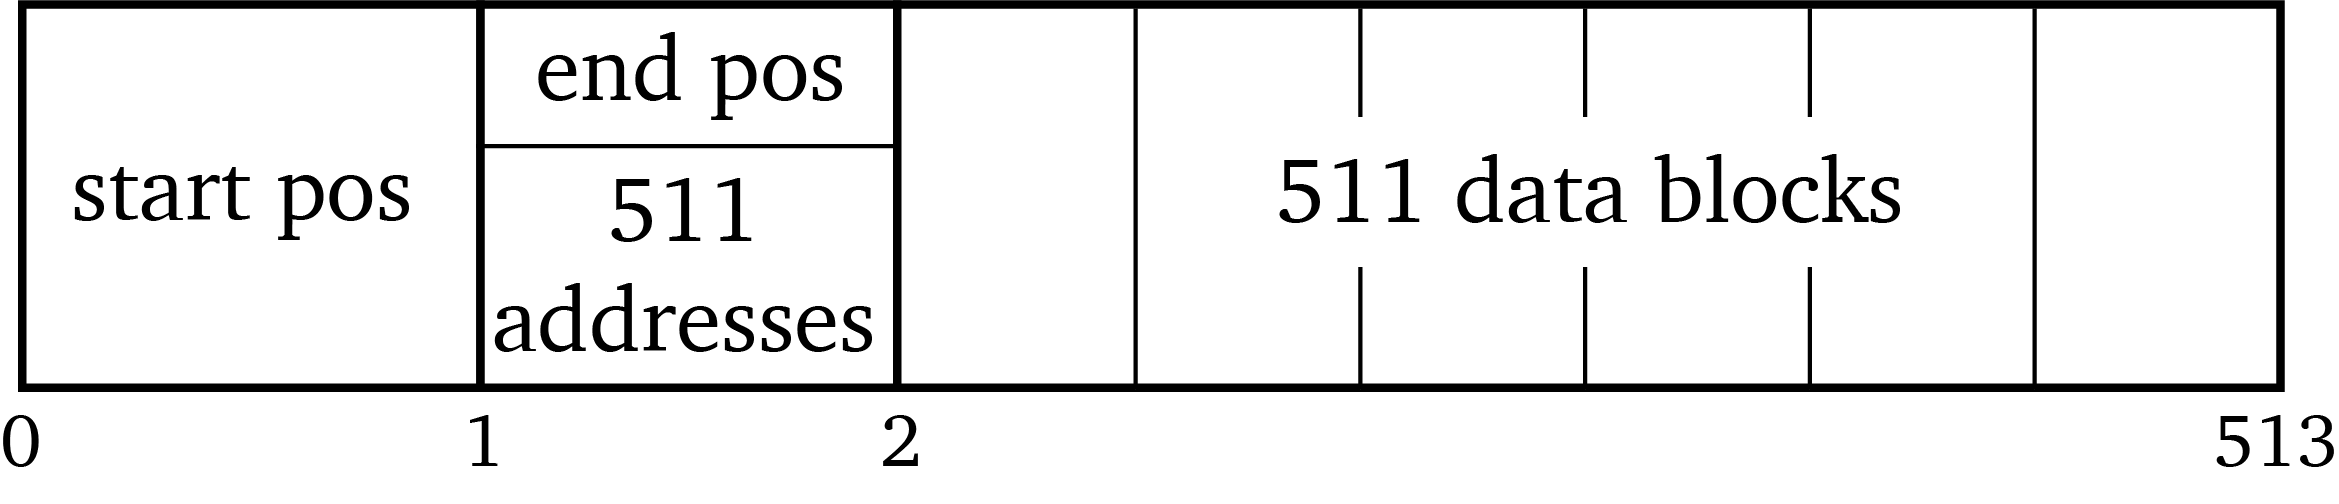
\includegraphics{fig/circ-phys.png}
\caption{The circular buffer's on-disk layout, consisting of a fixed 513 blocks
  located at the beginning of the disk.}
\label{fig:circ:phys}
\end{figure}

The basic idea is that the circular buffer is specified in terms of an abstract
state that transitions for each operation. The recovery operation
restores the pre-crash state of the queue from disk. The state for this library consists
of two components: a queue of updates (which are pairs of an address to write to
and a 4KB block to write there) and a 64-bit start position that indicates how
many updates occurred prior to the current list of updates. The \cc{Append} operation, as
mentioned, simply appends to the list of updates. The argument to \cc{TrimTill}
is an absolute position; the effect of \cc{TrimTill(pos)} is to delete
\cc{pos - start} updates from the beginning of the list of updates and set the
new start position to \cc{pos}. A more formal specification is given in
\cref{fig:circ:spec}.

The circular buffer supports atomic and concurrent \cc{Append} and \cc{TrimTill}
with a careful on-disk layout. It consists of two header blocks and 511 data
blocks, depicted graphically in \cref{fig:circ:phys}. The first header block
(the ``trim'' block, since it is used for trimming) holds the logical start
position of the queue, while the second header (the ``append'' block, since it
is used for appending) holds the logical end position and 511 addresses; the
data blocks for these addresses are in the remaining data blocks. This append
header has 4096 bytes, or enough space for 512 64-bit numbers; one is used for
the end position, and the remainder for update addresses. Recovery uses the
header blocks to determine what subset of the circular buffer holds complete
multiwrites; partially-appended updates are ignored for atomicity.

To append atomically, \cc{c.Append(end, upds)} first writes the data (using
\cc{end} to know where to start writing), and then writes the append header
block to atomically incorporate the writes, and simultaneously to write the
addresses. The in-memory \cc{c *Appender} struct keeps track of the existing
addresses so they can be re-written to disk. Meanwhile \cc{TrimTill} logically
deletes by merely writing a new, higher start position to the trim header.

Since these operations touch disjoint parts of disk, they can be performed
concurrently. However, one subtlety is that it is important to preserve the
queue abstraction that append operations do not overflow the circular buffer
(since this would overwrite old values) and that trim operations do not delete
past the current end (this would invalidate future appends immediately). The
insight that allows the caller to guarantee these properties is that the start
and end positions of the circular buffer are monotonically increasing, meaning
any snapshot of their positions is a \emph{lower bound} that is valid from then
on. Thus without holding any locks a call to \cc{c.TrimTill(newStart)} can
guarantee that the trim fits by showing that $\cc{newStart} \leq \cc{end_lb}$,
where \cc{end_lb} is merely a lower bound and not necessarily the exact end
position. However, it is necessary for the caller to know the exact start
position and that it will not change concurrently, in order to guarantee that
\cc{newStart} is greater than the current \cc{start}. The proof of
\cc{c.Append(end, upds)} is the dual of trim, requiring a lower bound on the
start position and exact control over \cc{end}.

\begin{figure}[ht]
\begin{minted}{coq}
(* Circular buffer Coq specification *)

Definition update := u64 * Block;
Record circ_state := {
  upds: list update;
  start: u64;
}.

(* requires length s.(upds) + length new_upds <= 511 *)
Definition append (s: circ_state) (new_upds: list update) : circ_state :=
  s <[ upds := s.(upds) ++ new_upds ]>.

(* requires s.(start) <= new_start *)
Definition trim_till (s: circ_state) (new_start: u64) : circ_state :=
  let num_removed := new_start - s.(start) in
  s <[ start := new_start ]>
    <[ upds := drop num_removed s.(upds) ]>.
\end{minted}
  \caption{The specification for the circular buffer, described as transitions
    on the abstract state.}
  \label{fig:circ:spec}
\end{figure}


There are three challenges in specifying how the circular buffer's
implementation connects to the abstract transitions given above. First, we
want to show that \cc{Append} appears to be atomic to the caller, even though
its implementation writes many disk blocks and the system could crash after
persisting only some of them. Second, the library has some thread-safety
requirements to enforce on the caller: in particular \cc{Append} and
\cc{TrimTill} can be called concurrently from separate threads, but it is not
safe to concurrently issue multiple appends or multiple trim requests. Finally, the library
relies on the caller to guarantee that \cc{Append} and \cc{TrimTill} are called with enough
available space. These last two challenges are due to leaving concurrency
control to the caller, which is more efficient than the circular buffer having
its own redundant locking.

The write-ahead log uses the circular buffer from two threads, one dedicated to
\emph{logging} which appends to the circular buffer to make writes durable and another
dedicated to \emph{installation} which trims writes from the circular buffer
after installing them. Appending and trimming can be performed concurrently, but
appending requires the \cc{*Appender} struct which is not thread-safe. The
caller only reads from the circular buffer if the system crashes, at which point
recovery restores the previous state.

\section{Circular buffer custom resources}

Perennial, like Iris, has support for user-defined separation-logic resources.
These are defined using lower-level mechanisms, but this section simply presents the
resources and the intuition for how they are used without going into details on
how they are implemented. The circular buffer defines and issues the
following custom separation-logic resources:

\newidentmacro{length}
\newcommand{\circstate}{\cc{circ_state}}
\newcommand{\startIs}{\cc{start_is}}
\newcommand{\diskendIs}{\cc{end_is}}

\begin{itemize}
  \item $\circstate(\gamma, \sigma)$, which says that the current state
  of the circular buffer is $\sigma$. The $\gamma$ argument is a ``ghost name''
  for the ghost state associated with this instance of the circular buffer; at
  any time there is only one circular buffer, but this name will change every
  time the system crashes and reboots and thus distinguishes different
  ``generations'' of the circular buffer.
  \item $\cc{is_circular}(\gamma)$, defined to be
  $\knowInv{}{\exists \sigma, \circstate(\gamma, \sigma) * P(\sigma)}$.
  The $P(\sigma)$ part of this invariant is part of the HOCAP specification
  style, explained below.
  \item $\cc{circ_appender}(\gamma, \ell)$. This relates the circular buffer's
  ghost state with $\ell$, a \cc{*circularAppender} pointer that has some data
  needed to append to the circular buffer. This resource is not persistent and
  is owned by the logger thread.
  \item $\startIs(\gamma, \cc{start})$ and
  $\diskendIs(\gamma, \cc{end})$ give the exact current positions of the start
  and end (that is, $\sigma.\cc{start} + \length(\sigma.\cc{updates})$) of
  the circular buffer. These resources are not persistent and are owned by
  the installer and logger threads respectively.
  \item $\cc{start_at_least}(\gamma, \cc{start})$ and
  $\cc{end_at_least}(\gamma, \cc{end})$ give \emph{lower bounds} on the start
  and end positions. It is possible to issue such resources because the start and
  end monotonically increase. As a result of monotonicity, these resources are
  persistent; once \cc{start} or \cc{end} reaches some value, that value is
  always a valid lower bound.
\end{itemize}

\section[Specifications for Append and TrimTill]%
{Specifications for \cc{Append} and \cc{TrimTill}}

Formally the way each operation is specified is using a style called
higher-order concurrent abstract predicates (HOCAP)~\cite{svendsen:hocap,jacobs:logatom}. The basic idea is that the
library maintains an invariant $P(\sigma)$, where $\sigma$ is the current
abstract state; a key idea in the HOCAP specification is that this predicate $P$
is chosen by \emph{the client} (that is, the code calling the library).

The predicates in HOCAP specifications express ownership over ghost state. This
aspect of Perennial is inherited from Iris and described in more detail in
\cref{sec:perennial:concurrency}. In this chapter we use the \emph{view-shift
assertion} $R \vs Q$ to express ghost updates, which are used to update the
predicate $P(\sigma)$ that the library maintains.\footnote{Note that this is a slight
notation shift, compared to the update modality used in the Perennial chapter; the view shift is equivalent to
$R \wand \upd Q$.} The intuition for $R \vs Q$ is that it represents some
resources which allow the holder of the assertion to take
$R \sep (R \vs Q)$ and ``fire'' the view shift, updating the underlying ghost
variables, and finally obtain $Q$.

For each operation, the client passes in a
view-shift $P(\sigma) \vs P(\sigma') * Q$, for any
transition from $\sigma$ to $\sigma'$ that is a valid transition for the operation.
This view shift represents a kind of once-usable ``callback'' which transforms
$P(\sigma)$ into $P(\sigma')$, by updating the caller's ghost state in
$P$. At the end of the operation, the client receives $Q$ as a kind of
certificate that the callback ran. The intuition here is that the library's proof must
``fire'' or ``call'' the view shift in order to preserve $P$ and produce $Q$,
but the proof gets to pick the exact moment when it should fire the view shift,
which is the linearization point of the operation. Note that the view shift
might be proven using exclusive resources that cannot be duplicated, so it is
important that it is only fired once.

We can see both the HOCAP pattern and the circular-buffer resources in action in
the specification for Append:
%
\begin{align*}
  &\{ \cc{is_circular}(\gamma) \sep {} \\
&\quad (\forall \sigma, P(\sigma) \vs P(\sigma \lappend \cc{upds}) * Q) \sep {} \\
&\quad \cc{circ_appender}(\gamma, \cc{c}) \sep {} \\
&\quad \diskendIs(\cc{end}) \sep \cc{start_at_least}(\cc{start}) \sep (\cc{end} - \cc{start} + \length(\cc{upds}) \leq 511) \\
&\} \\
&\qquad\cc{c.Append(end, upds)} \\
&\{ \cc{circ_appender}(\gamma, \cc{c}) \sep {} \\
&\quad \diskendIs(\cc{end} + \length(\cc{upds})) \sep Q \}
\end{align*}

There are several aspects to the specification, mostly in the precondition. The
first line is the most straightforward: we need the circular buffer's invariant
to hold, for a particular ghost name $\gamma$. The second line is part of the
general HOCAP pattern. The view shift updates $P(\sigma)$ to the appropriate new
state, denoted with $\sigma \lappend \cc{upds}$ as shorthand for $\sigma$ with \cc{upds}
appended to the updates field (and the same \cc{start}). The proof of this
specification executes the view shift at the linearization point of the \cc{Append}
operation, changing the state inside the $\cc{is_circular}$ invariant. The view
shift produces a client-supplied assertion $Q$, which is returned in the
postcondition.

The assertion $\cc{circ_appender}(\gamma, \cc{c})$ asserts that the
in-memory state cached in \cc{c} is correct (these are the addresses for the
updates but not their contents). This resource is unique, since the appending
thread needs ownership this in-memory buffer, and is returned in the
postcondition for the next \cc{Append} operation. Exclusive ownership over this
buffer is one reason why appending is only safe from one thread.

The rest of the specification is specific to how the circular buffer manages
concurrency. Appending requires precise knowledge of the end position of the
circular buffer, which the logger thread maintains. A lower bound on the start
position is sufficient to prove that there is currently---and will continue to
be---enough space for the updates to fit on disk; the left-hand side of the
inequality computes an \emph{upper bound} on how much space will be used after
the append because the \cc{start} variable is a lower bound. The postcondition
gives the caller back the $\diskendIs$ assertion with the new precise end point.
Note that the precondition guarantees that the append will not fail due to
running out of space. Because the start and end are manipulated without locks
the circular buffer implementation does not even have a way to safely
dynamically check if there is enough space.

The specification for \cc{TrimTill} is similar to Append:
%
\begin{align*}
  &\{ \cc{is_circular}(\gamma) \sep {} \\
&\quad (\forall \sigma, P(\sigma) \vs P(\sigma[:\cc{newStart}]) * Q) \sep {} \\
&\quad \startIs(\cc{start}) \sep \cc{end_at_least}(\cc{end}) \sep (\cc{start} \leq \cc{newStart} \leq \cc{end}) \\
&\} \\
&\qquad\cc{c.TrimTill(newStart)} \\
&\{ \startIs(\cc{newStart}) \sep Q \}
\end{align*}

The effect of a \cc{TrimTill}, abbreviated $\sigma[:\cc{newStart}]$, is to set
the start position and delete the first $\cc{newStart} - \cc{start}$ updates.
For this operation to be safe, it requires
that the start not go backwards (recall the Append proof relies on a lower bound
for \cc{start}) and not go past the current end position (concretely this would
logically delete updates that haven't yet been written!). The precondition
encodes these by taking a precise current \cc{start} position and a lower bound
on the end, and then requiring the new start variable be between the two. Just
like with Append, the installer thread that calls this operation always
maintains precise knowledge (ownership) of the start of the circular buffer.

Notice that neither of these specifications have a crash condition. The reason
this is not required is because both methods already maintain an Iris invariant in
the \cc{is_circular} predicate. The next
section,~\ref{sec:perennial:recovery-spec}, details how crashes and recovery are
specified in Perennial.

\section{Crash and recovery reasoning}%
\label{sec:perennial:recovery-spec}

The strategy behind proving crash safety is to prove a theorem about running a
whole system, restarting after every crash. For example, for DaisyNFS this
theorem applies to the server's main loop that receives a message from the
network, processes it in a background thread, and replies over the network.
Immediately following boot, before processing any requests, the server runs a
recovery procedure to restore in-memory state. This whole procedure --- recovery
followed by running the system --- is given an idempotent specification that is
proven with \ruleref{wpr-idempotence} from \cref{sec:perennial:recovery}. The
crash condition for this theorem is a description of the state of the whole
system at any intermediate step; describing this directly would be daunting, but
it is doable since each layer describes its part of the crash condition.

The circular buffer is the lowest layer of the implementation, so the way it
fits into the larger plan is that the whole system's recovery starts by
recovering the circular buffer's state, then uses that state to recover the next
layer, and so on until the whole system is ready to run. Schematically this
looks like the following:
%
\begin{minted}[linenos]{go}
func RunSystem() {
  c, start, upds := RecoverCircular()
  // recover rest of system from c, start, upds
  fs := recoverFilesystem(...)
  for {
    req := GetRequest()
    go func() {
      ret := fs.Handle(req)
      SendReply(req, ret)
    }()
  }
}
\end{minted}

The circular buffer supplies three things to fit into the whole-system
recovery proof: (1) an abstract crash predicate for the state the circular
buffer requires for recovery, (2) a crash specification for the circular
buffer's recovery procedure itself, and (3) a post-recovery init theorem that
helps the caller maintain the circular buffer's crash predicate and also
initializes the circular buffer's invariant.

The specification for the library's recovery procedure \cc{RecoverCircular()} is:
%
\begin{align*}
  &\{ \circstate(\gamma, \sigma) \sep \cc{circ_resources}(\gamma) \} \\
  &\qquad\cc{RecoverCircular()} \\
  &\{ \Ret{(\ell, \cc{diskStart}, \cc{upds})} \sigma = (\cc{diskStart}, \cc{upds}) \sep {} \\
  &\quad \circstate(\gamma, \sigma) \sep {}  \\
  &\quad \startIs(\cc{diskStart}) \sep \diskendIs(\cc{diskStart} + \cc{len}(\cc{upds})) \sep {} \\
  &\quad \cc{circ_appender}(\gamma, \ell) \} \\
  &\{ \circstate(\gamma, \sigma) \sep \cc{circ_resources}(\gamma) \}
\end{align*}
%
The first thing to notice about the recovery specification is that it preserves
$\circstate(\gamma, \sigma)$, which gives the current state of the circular
buffer, both on crash and if recovery completes. It is also the case that
$\cc{circ_appender}(\gamma, \ell) \proves \cc{circ_resources}(\gamma)$, so that
$\cc{circ_resources}(\gamma)$ is also preserved by recovery. These two together
are the crash predicate for the circular buffer. We say the crash predicate is
abstract because the user of this theorem does not need to know how it is
defined.

\newcommand{\cfupdw}{\mathrm{cfupd}}
\newcommand{\cfupd}[1]{\cfupdw\left(#1\right)}
\newcommand{\cinvw}{\mathrm{cinv}}
\newcommand{\cinv}[1]{\mathrm{cinv}\left(#1\right)}

The circular buffer's proof also supplies the following \emph{post-recovery
init} theorem, which sets up the circular buffer for use after recovery:
%
\begin{align*}
  &\forall \sigma, P(\sigma) \vs %
  P_{\mathrm{rec}}(\sigma) \sep %
  P_{\mathrm{crash}}(\sigma) \proves \\
  &\circstate(\gamma, \sigma) \sep P(\sigma) \vs \\
  &\exists \gamma'.\, \cc{is_circular}(\gamma) \sep {} \\
  &\quad \cfupd{ \exists \sigma.\, \circstate(\gamma', \sigma) \sep %
    \cc{circ_resources}(\gamma', \sigma) \sep %
    P_{\mathrm{rec}}(\sigma) } \sep {} \\
  &\quad \cinv{ \exists \sigma.\, \circstate(\gamma, \sigma) \sep %
    \cc{circ_exchanger}(\gamma, \gamma') \sep %
    P_{\mathrm{crash}}(\sigma) }
\end{align*}

There are several components to this theorem. First, the circular buffer has the
caller provide a way to split the HOCAP predicate $P(\sigma)$ into two parts,
$P_{\mathrm{rec}}(\sigma)$ and $P_{\mathrm{crash}}(\sigma)$ --- intuitively the
former is transferred to recovery as part of its precondition, whereas the
latter is ``immutable'' and held inside an invariant. Second, the theorem
consumes $\circstate(\gamma, \sigma) \sep P(\sigma)$ and allocates three things:
(1) $\cc{is_circular}(\gamma)$ (notice that the \cc{is_circular} is defined to
be an invariant, and the premise of this theorem is the contents of that invariant), (2) a ``$\cfupdw$'', and a (3) ``$\cinvw$''. The
latter two are low-level features of Perennial that we'll now introduce.

The assertion $\cfupd{R}$ (``crash fancy update'') is similar to a view-shift
$\TRUE \vs R$ in that it is a single-use update that produces the resources $R$.
However, the ``crash'' part indicates that this update can only be fired after a
crash, so it can be used to prove a crash condition but is otherwise unusable.
Practically speaking, having $\cfupd{R}$ in a precondition allows the user to
\emph{cancel} $R$ from the proof's crash condition, as reflected in the
following rule:

\begin{mathpar}
  \inferH{cfupd-use}
  {P \proves \wpc{e}{Q}{Q_{c}}}%
  {P \sep \cfupd{R} \proves \wpc{e}{Q}{Q_{c} \sep R}}
\end{mathpar}

In the context of the circular buffer, what the $\cfupdw$ sets up for the caller
is that if the system crashes, the recovery proof can dismiss the circular
buffer's crash predicate, along with $P_{\mathrm{rec}}(\sigma)$, from the
overall crash condition. Thus using \ruleref{cfupd-use} before running the
system both sets up the circular buffer for use (by establishing
$\cc{is_circular}(\gamma)$) and guarantees the circular buffer's part of the
crash condition from now on. A simpler but abstract version of this
reasoning appears in the \ruleref{wpc-inv-alloc} rule in \cref{sec:perennial:wpc};
this theorem is a concrete use case (split into creating the cfupd and later
using it, rather than in one step as in \ruleref{wpc-inv-alloc}). What Perennial
makes possible is to take advantage of the invariant for crash reasoning ---
what must be carefully handled is that while the invariant is shared by all
threads, only one thread can get ``credit'' for this invariant holding at crash
time, in the sense of permission to cancel it from its crash condition.

Notice in the circular buffer's post-recovery init theorem that the ghost name
for the circular buffer changes on crash to a new $\gamma'$; the reason for this
is that other threads (the logger and installer) have access to some of the
circular buffer resources associated with $\gamma$. Rather than requiring those
threads to ``return'' those resources on crash and impose a crash condition on
that code, this theorem simply creates a new instance of the circular buffer and stops using
the old one. As a result on crash the theorem can produce
$\cc{circ_resources}(\gamma', \sigma)$ and hand out these resources to the
caller.

The third component of the theorem is a $\cinvw$ (``crash invariant'').
$\cinv{R}$ behaves very similarly to an invariant assertion $\knowInv{}{R}$, except
that like a crash fancy update it can only be used after a crash. This crash
invariant ``freezes'' the old state of the circular buffer (notice that
$\circstate(\gamma, \sigma)$ is now unchanging, since future operations will
interact with the instance named $\gamma'$). This process also produces
$\cc{circ_exchanger}(\gamma, \gamma')$, which includes additional ghost state
relating the old and new instances in the form of the predicate. The circular buffer in
particular does not have an interesting exchanger predicate, but this feature of
the specification pattern shows up in the GoTxn proof.

In general, each layer supplies a post-recovery init theorem. The view shift for
each of these
theorems is invoked in the proof of a program like \cc{RunSystem()} after
running all the recovery code and just
before normal processing (after line 4 in the code above). Firing these view shifts allocates all the layers'
invariants while simultaneously getting credit for this allocation in the
form of the $\cfupdw$ assertions, similar to how \ruleref{wpc-inv-alloc} works.
Prior to calling this initialization, the recovery procedure has access to the
inner contents of all the invariants, reflecting that it has exclusive access,
but in turn this proof is required to maintain a complicated crash condition.
(One interesting side effect is that recovery code can safely call library
functions without using locks, since this code is still guaranteed to be
single-threaded.) Once the system starts running the invariant allows multiple
threads to share access to this state, and the invariant implicitly guarantees
the crash condition recovery depends on.

\section{Exchanging resources}%
\label{sec:perennial:exchanging}

The final aspect of the logically-atomic specification pattern is the role of
the exchanger, one of the conclusions of the post-recovery init theorem. The
purpose of this predicate is to give the caller a way to, on crash, relate
resources issued by the library before a crash to those after a crash. In the
circular buffer, the $\startIs(\cc{start})$ and $\diskendIs(\cc{end})$ resources
are thrown away on crash and re-created during recovery; there are only two of
them, so it is easy enough to reconstruct them globally. In contrast, some
resources are used locally by a thread and we would like a way to retain
ownership across a crash, into that thread's crash condition. This is exactly
what happens with GoTxn's lifting-based specification for the journaling layer, explained in greater
detail in \cref{sec:txn:lifting}. Exchanging gives threads a way to ``trade''
ownership during a crash, trading ownership associated with the old $\gamma$ instance for
associated with $\gamma'$; both forms of ownership can be
exclusive because the process destroys the old ownership and thus can only be
performed once.

\newcommand{\mapstoDisk}{\mapsto_d}
\newcommand{\mapstoOp}{\mapsto_{\mathit{op}}}
\newcommand{\mapstoLftd}{\mapsto_d^{\mathrm{lftd}}}
\newcommand{\jrnlToken}[1]{\textlog{token}(#1)}

To make this a bit more concrete, let us look at a part of the GoTxn lifting
specification. This specification issues three related resources: the two more important
ones are $a \mapstoDisk o$ and $a \mapstoOp o$. Both represent exclusive
access to address $a$. $a \mapstoDisk o$ is a durable statement about the
logical disk, while $a \mapstoOp o$ gives the value at address $a$ that
an in-progress operation $op$ would observe. The lifting-based specification
gets its name from a logical ``lift'' operation that trades $a \mapstoDisk o$
for $a \mapstoOp o \sep a \mapstoLftd o$. This brings us to the
third type of GoJournal resource, $a \mapstoLftd o$, which is
almost identical to $a \mapstoDisk o$ except that it has been lifted and thus
cannot be lifted again.\footnote{In the implementation,
$a \mapstoLftd o$ is the primitive resource. There is a
resource $\jrnlToken{a}$ that gives the right to lift $a$. Then
$a \mapstoDisk o$ is simply defined to be
$a \mapstoLftd o \sep \jrnlToken{a}$.} We can give
the journal's \cc{Commit} operation a
specification like the following (simplified, in particular to operate on a
single address):
%
\begin{align*}
  \hoareCV{a \mapstoLftd o \sep a \mapstoOp o'} %
  {\mathit{op}.\cc{Commit}()}%
  {\Ret{\mathit{ok}} \mathrm{if~} \mathit{ok} %
  \mathrm{~then~} a \mapstoDisk o' \mathrm{~else~} a \mapstoDisk o}%
  {a \mapstoDisk o \lor a \mapstoDisk o'}
\end{align*}

In the non-error, non-crash return, the postcondition turns $a \mapstoOp o'$
into a durable fact $a \mapstoDisk o'$. If the system doesn't crash but the
transaction fails (which happens if it is too large to fit in the circular
buffer), then the caller gets back an unlifted disk fact $a \mapstoDisk o$,
reflecting that the transaction did not affect the disk. In the case of a crash
the specification promises to give one of these assertions, and which one
depends on exactly when the crash occurs.

This specification is simplified to only give the case of committing an
operation that modifies a single address, when in reality \cc{Commit}'s main purpose
is to atomically commit multiple addresses; a single address is enough to
understand the proof issues involved. If the system doesn't crash, it is
relatively straightforward to reverse the lifting process and restore full
ownership of the disk values. $a \mapstoDisk o'$ reflects that the commit
actually succeeded in changing the disk value, while $a \mapstoDisk o$ results
from aborting and throwing away buffered writes in $op$.

On crash it is more difficult to show $a \mapstoDisk o \lor a \mapstoDisk o'$.
The challenge is how to propagate whether or not the writes were made durable
from the lower-level abstractions up to this proof; indeed the durability of
this high-level operation depends on whether or not the lowest level of the
system, the circular buffer, successfully wrote a single header block!

The write-ahead logging layer conveys durability by issuing two resources: one
gives the history of multiwrites, and another gives a lower bound on how many
multiwrites are durable. Its exchanging resource allows the caller to trade an
assertion about the history before a crash for a similar assertion after a
crash, albeit with some recent writes lost. Crucially the effect of a crash is
constrained by the durable lower bound, which can also be exchanged across a
crash. On top of this exchanging, the journaling proof implements a fine-grained
exchange of ownership over individual addresses.

The actual implementation of exchanging uses a neat separation logic trick. To
distinguish between $a \mapstoDisk o$ in two different generations, we'll
annotate the resource with a $\gamma$. The exchanger for the journaling proof is
defined in terms of facts like:
\[
  \cc{exchange_addr}(a) \defeq (a \mapsto^{\gamma, \mathrm{lftd}}_{d} o) \lor (a \mapsto^{\gamma'}_{d} o)
\]
When proving the post-recovery init theorem, we initially prove
$\cc{exchange_addr}(a)$ using the right-hand side; this is easy since $\gamma'$
is fresh, so we've just allocated all of its associated ghost state and it
hasn't been used by any threads so far. We can then prove exchange lemmas like
$a \mapsto^{\gamma, \mathrm{lftd}}_{d} o \sep \cc{exchange_addr}(a) \proves a \mapsto^{\gamma'}_{d} o \sep \cc{exchange_addr}(a)$.
The reason this proof works is that $a \mapstoLftd o$ is \emph{exclusive}, thus
from the premise the proof can rule out that $\cc{exchange_addr}(a)$ is proven with the
left disjunct and learn that the right-hand side holds. The proof takes out this
right disjunct ($a \mapsto^{\gamma'}_{d} o$) and gives up
$a \mapsto^{\gamma, \mathrm{lftd}}_{d} o$ to re-prove $\cc{exchange_addr}(a)$, this time using
the left disjunct. This all ensures that exchanging is only performed once,
which is necessary since all the resources involved are exclusive.

There is an important asymmetry here where the old ghost state only requires
$a \mapstoLftd o$ while exchanging returns $a \mapsto_{d} o$. This asymmetry is
possible because $a \mapsto_{d} o$ is just like $a \mapstoLftd o$ but with an
additional exclusive token that gives the right to lift the address, and we can
``drop'' the old tokens in the proof and switch to using fresh tokens generated
for $\gamma'$. In practice this is what permits proving the \cc{Commit}
operation's crash condition that has $a \mapsto_{d} o$ when the specification's
precondition only has $a \mapstoLftd o$.

% look at \cc{exchange_mapsto_commit} for the interesting case (ephemeral values
% that might now be durable) and \cc{exchange_durable_mapsto} for the
% straightforward case (durable values that are now proven to still be durable,
% exchanger shows old lower bounds are still valid)

\section{Summary}

The overall logically-atomic crash specification pattern has four components for
every layer of the system:

\begin{itemize}
  \item An opaque predicate for the abstract state of the system (e.g.,
        $\circstate(\gamma, \sigma)$).
  \item Proofs for each operation that use a client-specified predicate,
        modified by requiring a view shift that updates the predicate in
        accordance with the operation's effect on abstract state.
  \item An opaque crash predicate for the system.
  \item A recovery theorem, with a crash condition, that preserves the crash
  predicate for the system and re-builds any in-memory state needed.
  \item A post-recovery init theorem, to be called after the whole system has
        recovered, which sets up the layer's invariant for normal execution,
        creates ghost state for the next generation, and produces an exchanger
        resource to relate the old state to the new one.
\end{itemize}

When layers are composed, the upper layer proof generally hide the lower level
in its own proofs --- for example, the write-ahead log's crash predicate
includes the circular buffer's crash predicate as a sub-term, and subsumes the
circular buffer's recovery and post-recovery init theorems.

This pattern can be combined with user-defined ghost resources in order to give
more powerful specifications (rather than requiring every operation to be
unconditionally atomic). User-defined ghost resources can interact with crashes
and recovery; for example, they can be returned from the recovery theorem and
used across a crash using exchanging lemmas specific to the library.

